\documentclass[runningheads,a4paper]{llncs}

\usepackage{amssymb}
\setcounter{tocdepth}{3}
\usepackage{graphicx}

\usepackage{url}
\urldef{\mailsa}\path|{qian_chen}@sjtu.edu.cn|
\newcommand{\keywords}[1]{\par\addvspace\baselineskip
\noindent\keywordname\enspace\ignorespaces#1}

\begin{document}

\mainmatter

\title{ Affective Recognition Using EEG Signal in Human-robot Interaction }
\titlerunning{ Affective Recognition Using EEG Signal in Human-robot Interaction}

\author{Chen Qian\and Tingting Hou\and Shan Fu }

\authorrunning{ Affective Recognition Using EEG Signal in Human-robot Interaction}
\institute{School of Electronic Information and Electrical Engineering, Shanghai Jiao Tong University,
Shanghai, 200240, P.R. China\\
\mailsa }

\maketitle
%Abstract
\begin{abstract}
TODO : this part is waiting to be rewritten.
\keywords{Affective Computing; Arm-Robot Operation; Time Domain Features;
Domain Feat}
\end{abstract}

\section{Introduction}
Hitherto, mechanical arm, as a vital product in industry field, has been broadly
used in medical, exploration, rescue field etc. However, the mistake operation
caused by human error, which should have been avoided, is still one of the
dominant reasons causing accidents. As we all know, the state of human has a
close link to the cognitive state of human and in some degree emotion is the
main reason causing the change of the cognitive state, therefore, one of
critical ways to avoid huamn error in mechanical arm operation is recognizing
the emotion during the opreration process through detecting the physiological
signal. Since R. W. Picard has defined Affective Computing $(AC)^{\cite{AC}}$
in 1995, affective computing has been a critical field in human-computer
interaction area.  such as Blood Volume Pressure (BVP), Skin Conductance
Response (SCR), Respiration (RESP), Electrocardiogram (ECG), Electromyogram (EMG),
Electrocorticogram (ECoG), Electroencephalogram (EEG), Heart Rate (HR), Oxygen
Saturation (SaO2) and Surface Temperature (ST)\cite{KR}. In all physiological
signals, EEG is no doubt the most capable signal directly reflecting the brain
activity. Therefore this paper chooses to use 32 dry electrodes EEG signal acquisition
equipment to obtain EEG signal data during mechanical arm operation.


There are lots of models which has been proposed to describe the emotion, such as
six basic emotions model proposed by Ekman et al.\cite{Ekman}, eight basic emotions
model proposed by Plutchik\cite{Plutchik} and the valence-arousal scale proposed
by Russell\cite{Russell}. For simplifing this problem, this paper chooses to use the
valence in the valence-arousal model of Russell to evaluate the emotion of the subjects.
And the valence reflecting the positive or negative aspect of the subjects is enough
to describe the cognitive state of the subjects.


Besides the model of emotion, the way to obatain the ground truth of the subjects
is also crucial. Almost all research in Affective Computing field use the self-assessment
scores to estimate the true cognitive state of the subjects. However, even the subjects
themselves could hardly to retell the exact emotion state in the mechanical arm operation
and using one single scores to estimate the cognitive state during the entire operation process
 is obiviously not reasonable in detail. So this paper proposes to use objective and real time
 indexes to represent the cognitive state of the subjects. In this paper, we record the track
 of the end point of the mechanical arm and extract the features of the track to represent
 the fluctuation of the cognitive state of the subjects. Meanwhile, we assume that the workload
  and the time pressure could stimulate the emotion change of the subjects, so we give a
  basic score, which reflects the emotion state the subjects should be, and add the weighted
  features scores to the basic score to reflect the fluctuation of the emotion state.


In our experiment, we designed three levels of operating tasks in different difficulty to
  stimulate the emotion state change. And the level of difficulty is determined by the
  workload and the time pressure. To eliminate the influence of unfamilarity, one minute
  of free exploration is added before these three tasks and to eliminate the interaction
  of different tasks, a 30 seconds reset time interval is added between the different
  tasks.


During the data process part, because of the low signal-to-noise ratio (SNR),
the disturbance of EMG signal and the electromagnetic interference, the raw data
have firstly been filter to the 1-64Hz frequecy band\cite{Feature}. After normalization
process, different scales sliding window are induced in extracting features. Because of
the real-time label we obtain from the track mentioned above, it allows us to consider the
data in single sliding window as one sample.

The feature extraction methods are detailed summarized in papaer\cite{Feature}, we choose
three time domain features and one frequency feature to represent the raw data according
to the value of the weighted relative occurrence. And at the feature selection process,
we apply Principal Component Analysis (PCA) and Linear Discriminant Analysis (LDA) to
select the extracted features above. And at the classification design process, we apply
Support Vector Machine (SVM), which is a effective classification discriminator,
to predict the emotion state.

Here is the remainder organization of this paper: Section 2 introduce the
apparatus used in the experiment and the detail experiment protocol. Section 3
describes the data preprocess procedure, feature extraction, feature selection
classification design methods. Section 4 focus on showing the data process
results. Section 5 discusses the results. Section 6 gives the conclusion of
our experiment.
%mistake, Emotion is an important psychological process which could be induced by
%conscious and unconscious brain activities. This psychological process could
%reflect the cognitive state of , such as emotional images, musics, and video clips.
%Actually, many researching works have been done

\section{Experiment Setup}
\subsection{Apparatus}
There are 3 key equipment we use in our experiment: EEG Signal Acquisition Equipment,
Mechanical Arm and Joystick. And there are 3 personal computer for communicating
with EEG equipment, controling movement of mechanical arm through joystick and
showing the end point of the mechanical arm.
\paragraph{EEG Signal Acquisition Equipment:}
The EEG Signal Acquisition Equipment we apply is the Cognionics HD-72 Dry EEG
Headset(see in Fig.~\ref{fig:EEGequipment}).
Considering the difficulty of wearing EEG equipment and the comfort of the subjects,
we choose 32 dry electrodes to obtain the EEG signal, which are showed in


\begin{figure}
\centering
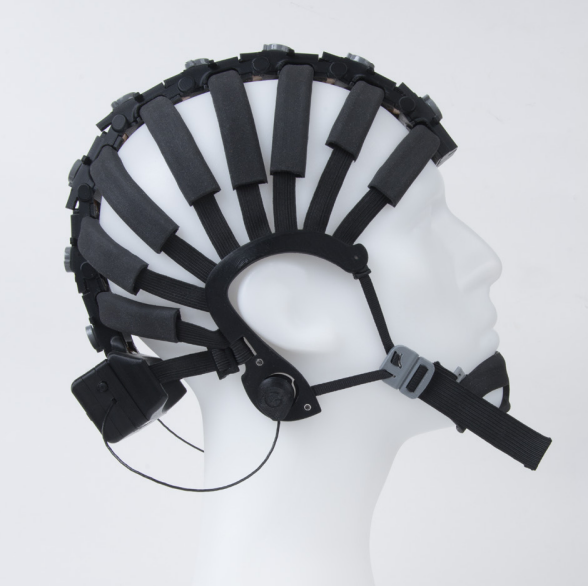
\includegraphics[height=6.2cm]{images/1}
\caption{}
\label{fig:EEGequipment}
\end{figure}


\subsection{Experiment Protocol}


\section{Data Process Method}

\subsection{Data Preprocess}
\subsection{Multi-scale Feature Extration}
\subsection{Feature Selection}
\subsection{Classification}

\section{Results}

\section{Discussion}

\section{Conclusion}



\begin{thebibliography}{4}

\bibitem{AC} Picard R W.
  Affective computing[M].
   MIT Press, 1997.

\bibitem{KR} Khosrowabadi R, Wahab A, Ang K K, et al.
Affective computation on EEG correlates of emotion from musical and vocal stimuli[C]
//Neural Networks, 2009. IJCNN 2009. International Joint Conference on. IEEE, 2009: 1590-1594.

\bibitem{Ekman} Ekman P, Friesen W V, O'sullivan M, et al.
Universals and cultural differences in the judgments of facial expressions of emotion[J].
Journal of personality and social psychology, 1987, 53(4): 712.

\bibitem{Plutchik} Plutchik R.
Emotions: A general psychoevolutionary theory[J].
Approaches to emotion, 1984, 1984: 197-219.

\bibitem{Russell} Russell J A.
A circumplex model of affect[J].
Journal of personality and social psychology, 1980, 39(6): 1161.

\bibitem{Feature} Jenke R, Peer A, Buss M.
Feature extraction and selection for emotion recognition from EEG[J].
IEEE Transactions on Affective Computing, 2014, 5(3): 327-339.

\bibitem{url} National Center for Biotechnology Information, \url{http://www.ncbi.nlm.nih.gov}

\end{thebibliography}

















\end{document}
